%%%%%%%%%%%%%%%%%%%%%%%%%%%%%%%%%%%%%%%%%
% Short Sectioned Assignment
% LaTeX Template
% Version 1.0 (5/5/12)
%
% This template has been downloaded from:
% http://www.LaTeXTemplates.com
%
% Original author:
% Frits Wenneker (http://www.howtotex.com)
%
% License:
% CC BY-NC-SA 3.0 (http://creativecommons.org/licenses/by-nc-sa/3.0/)
%
%%%%%%%%%%%%%%%%%%%%%%%%%%%%%%%%%%%%%%%%%

%----------------------------------------------------------------------------------------
%	PACKAGES AND OTHER DOCUMENT CONFIGURATIONS
%----------------------------------------------------------------------------------------

\documentclass[paper=a4, fontsize=11pt]{scrartcl} % A4 paper and 11pt font size

\usepackage[T1]{fontenc} % Use 8-bit encoding that has 256 glyphs
%\usepackage{fourier} % Use the Adobe Utopia font for the document - comment this line to return to the LaTeX default
\usepackage[english]{babel} % English language/hyphenation
\usepackage{amsmath,amsfonts,amsthm} % Math packages
\usepackage{bm}
\usepackage{lipsum} % Used for inserting dummy 'Lorem ipsum' text into the template
\usepackage{graphicx} % This one is for pictures
\usepackage{sectsty} % Allows customizing section commands
\allsectionsfont{\centering \normalfont\scshape} % Make all sections centered, the default font and small caps
\usepackage{color}

\usepackage{fancyhdr} % Custom headers and footers
\pagestyle{fancyplain} % Makes all pages in the document conform to the custom headers and footers
\fancyhead{} % No page header - if you want one, create it in the same way as the footers below
\fancyfoot[L]{} % Empty left footer
\fancyfoot[C]{} % Empty center footer
\fancyfoot[R]{\thepage} % Page numbering for right footer
\renewcommand{\headrulewidth}{0pt} % Remove header underlines
\renewcommand{\footrulewidth}{0pt} % Remove footer underlines
\setlength{\headheight}{13.6pt} % Customize the height of the header

\numberwithin{equation}{section} % Number equations within sections (i.e. 1.1, 1.2, 2.1, 2.2 instead of 1, 2, 3, 4)
\numberwithin{figure}{section} % Number figures within sections (i.e. 1.1, 1.2, 2.1, 2.2 instead of 1, 2, 3, 4)
\numberwithin{table}{section} % Number tables within sections (i.e. 1.1, 1.2, 2.1, 2.2 instead of 1, 2, 3, 4)

\setlength\parindent{0pt} % Removes all indentation from paragraphs - comment this line for an assignment with lots of text

%----------------------------------------------------------------------------------------
%	TITLE SECTION
%----------------------------------------------------------------------------------------

\newcommand{\horrule}[1]{\rule{\linewidth}{#1}} % Create horizontal rule command with 1 argument of height

\title{	
\normalfont \normalsize 
\textsc{Columbia University -- Fall 2013} \\ [25pt] % Your university, school and/or department name(s)
\horrule{0.5pt} \\[0.4cm] % Thin top horizontal rule
\huge Machine Learning Homework \#1\\ % The assignment title
\horrule{2pt} \\[0.5cm] % Thick bottom horizontal rule
}

\author{Joe Ellis} % Your name

\date{\normalsize\today} % Today's date or a custom date

\begin{document}

\maketitle % Print the title

%----------------------------------------------------------------------------------------
%	PROBLEM 1
%----------------------------------------------------------------------------------------

\section{Problem 1}

In this problem we investigate fitting a polynomial model and regression to a dataset consiting of 10 data points.  
Our $d$-dimensional polynomail function, $f$, is described below, 

\begin{align} 
f(x;\bm{\theta}) = \bm{\theta}_{0}	+ \bm{\theta}_{1}x_{1} + \bm{\theta}_{2}x_{2} + ... + \bm{\theta}_{d}x_{d}		
\end{align}

where $\bm{\theta}$ is the learned parameters of our model, and $x$ is a given data point.
We choose to use squared error for our empirical loss function to gauge how well our model fits the data present.  The equation for empirical loss can be seen below, where $x$ represents the given data points, $y$ represents the output, which our function $f$ is attempting to solve for.

\begin{align} 
R_{emp}(\bm{\theta}) = \frac{1}{N}\sum\limits_{i=1}^n (y_{i} - f(x_{i};\bm{\theta}))^{2}
\end{align}

We perform cross-validation to find the adequate dimensionality of an appropriate model.  
The cross-validation performed is completed 1000 times for each model complexity with train/test split of 9 points for training and 1 point for testing.  The results of the cross-validation can be seen in Figure 1., and we can see that a model of 4 or 5 dimesions is suitable for this dataset.  Models with lower than 3-dimensions have a hard time describing the variation in the data, where as models with many more than 3-dimensions tend to overfit.

\begin{figure}
\centering
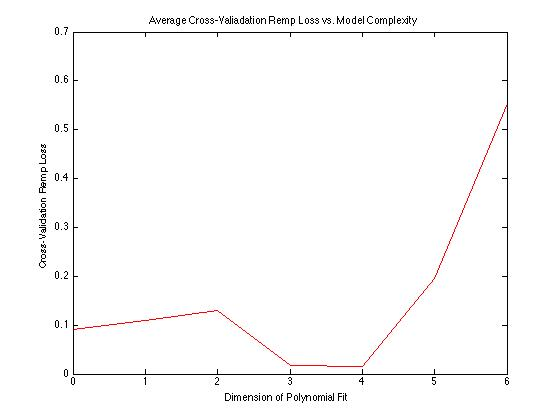
\includegraphics[scale=0.4]{Prob1_CrossValError.jpg}
\end{figure}

Using the 3-dimensional model for $f$ we achieve the best polynomial regression function with  with our $R_{emp}(\bm{\theta}) = 0.0046$, and $\bm{\theta} = (0.1951, 5.4884, -19.6041, 14.9130)$.

The plot of the polynomial that was found to fit the data set can be seen in Figure 2.

\begin{figure}
\centering
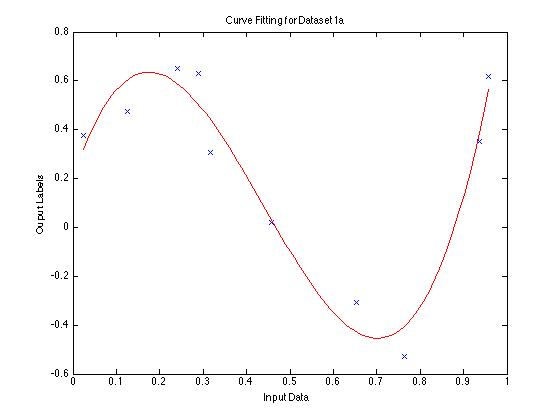
\includegraphics[scale=0.4]{Curve.jpg}
\end{figure}

\section{Problem 2}

In Problem 2 we also address the issue of finding some function to fit to a given set of data points and their real valued labels.  However, instead of using a standard polynomial basis function as described in Problem 1 we instead use a set of basis functions that consist of harmonic sets of $cos$ and $sin$ functions, 

\begin{align}
f(x;\bm{\theta}) = \theta_{0} +\sum\limits_{i=1}^k \theta_{i}sin(i*x) + \sum\limits_{i=1}^k \theta_{i+k}cos(i*x),
\end{align}

and these are known as sinusoidal basis functions.
The calculation of the sinusoidal regression function shown above was completed in the  ``sinusoidalreg.'' program, which was handed in with this assignment.  
The $R_{emp}(\bm{\theta})$ was calculated in the same way as above.
For this problem we once again used 1-dimensional input data with real valued output variables from ``dataset1b.txt'' that was provided to us.
For this dataset the first 100 elements from dataset1b were used for training and the second 100 were used for testing.
We completed 100-fold cross validation across the training set using a training/test split of 80 points for training and 20 for test to determine what was a good complexity for to model these data points.
A plot of the cross-validation accuracies can be seen below in Figure 3.

\begin{figure}
\centering
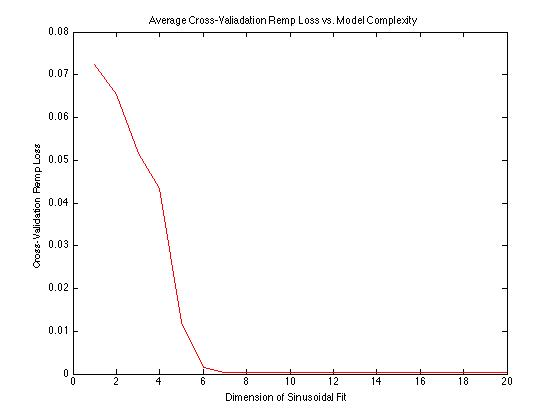
\includegraphics[scale=0.4]{Prob2_CrossValError.jpg}
\end{figure}

We can see that a good dimensionality for k that allows for a simple model but good performance, is $k=6$.  Using $k = 6$ as our model parameter we were able able to achieve a training error of $R_{emptrain} = 0.0012$ and testing error of $R_{emptest} = 0.0042$.  The found model has 13 parameters, and these parameters will be outputted to the screen if ``runProblem2.m'' is executed in the matlab command line environment, they were ommitted here for brevity.
Finally, the result of our sinusoidal regression function can be seen below in Figure 4, where points marked by an ``x'' are training points, and those marked by an ``o'' are test points.

\begin{figure}
\centering
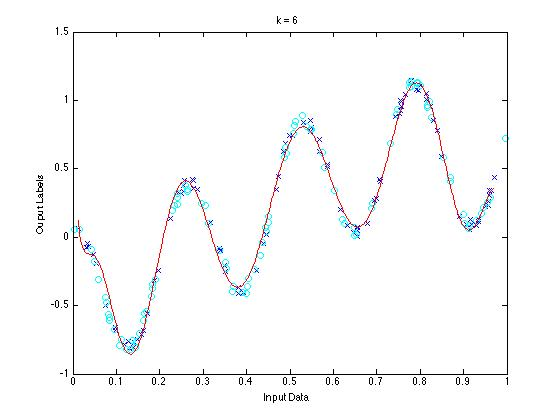
\includegraphics[scale=0.4]{prob2curve.jpg}
\end{figure}

\section{Problem 3}

In Problem 3 we will use a linear logistic regression function to perform a binary classification task on 2-D input data.  In this problem we find a suitable $\bm{\theta}$ for our logistic classification function by using batch gradient descent.  The logistic classification function is defined as, 

\begin{align}
f(x;\bm{\theta}) = \frac{1}{1+exp(-\bm{\theta}^t\bm{x})}.
\end{align}

For this problem instead of using the average squared error for our loss function instead we will use, the logistic loss cost function, which is defined as, 

\begin{align}
R_{emp}(\bm{\theta}) = \frac{1}{N}\sum\limits_{i=1}^N(y_{i}-1)log(1-f(x;\bm{\theta})) - y_{i}log(f(x;\bm{\theta})).
\end{align}

To perform gradient descent to find the global minimum of $R_{emp}(\bm{\theta})$ we need to find the partial derivatives of $R_{emp}(\bm{\theta})$ with respect to each different parameter within the $\bm{\theta}$ vector.  The partial with respect to each element of $\bm{\theta}$ is,

\begin{align}
\frac{\partial R_{emp}}{\partial \theta_{j}} = \frac{1}{N}\sum\limits_{i=1}^N(y_{i}-f(x;\bm{\theta}))x_{ij}.
\end{align}

Once we have the partial derivative for each element we can find the $\nabla R_{emp}(\bm{\theta})$, and then update our theta using this found gradient. 
We define a stepsize as $\eta = 100$, and then update our $\bm{\theta}$ after every iteration of gradient descent according to the equation,

\begin{align}
\bm{\theta} ^{t+1} = \bm{\theta} ^t + \eta*\nabla R_{emp}(\bm{\theta})
\end{align}

This algorithm completes once $| \bm{\theta} ^{t+1} -  \bm{\theta} ^t| < \epsilon$, where we have chosen $\epsilon = 0.1$. 
Using the gradient descent algorithm we were able to achieve a perfect binary classification error on the given dataset, and our algorithm converges to a solution after only 80 iterations.
The $\eta$ chosen allowed for very aggresive steps, and with this our Loss and binary error had some level of oscillation throughout the process.
Our final found normalized parameters give $\bm{\theta}  = (-0.319, 0.836, 0.444)$, with a $R_{emp}(\bm{x};\bm{\theta}) = 0.0146$ 
In Figure 6, we can see the  final linear logistic classifier imposed on top of our dataset, which shows the classification scheme.

\begin{figure}
\centering
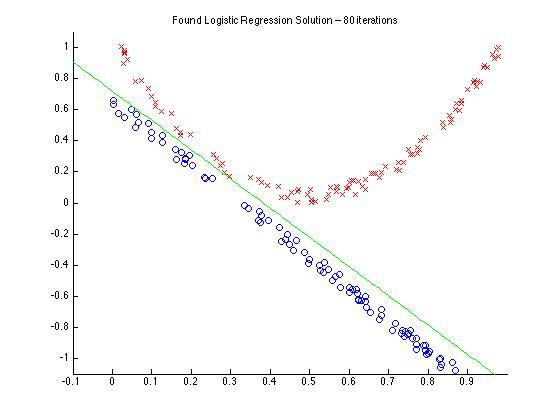
\includegraphics[scale=0.4]{prob3sol.jpg}
\end{figure}

Figure 7 demonstrates how the $R_{emp}(\bm{\theta})$ varies over the iteration process, notice the oscillations due to the large step size.

\begin{figure}
\centering
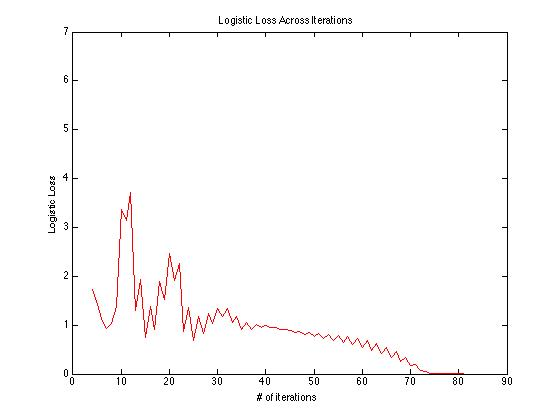
\includegraphics[scale=0.4]{logisticloss.jpg}
\end{figure}

Figure 8 shows how the Binary Classification error changes throughout the process.

\begin{figure}
\centering
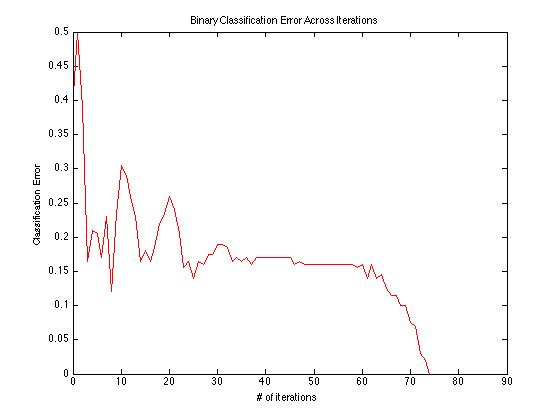
\includegraphics[scale=0.4]{BinClassErr.jpg}
\end{figure}

The $| \bm{\theta} ^{t+1} -  \bm{\theta} ^t|$ measure can be seen for every step in the iteration in Figure 9.

\begin{figure}
\centering
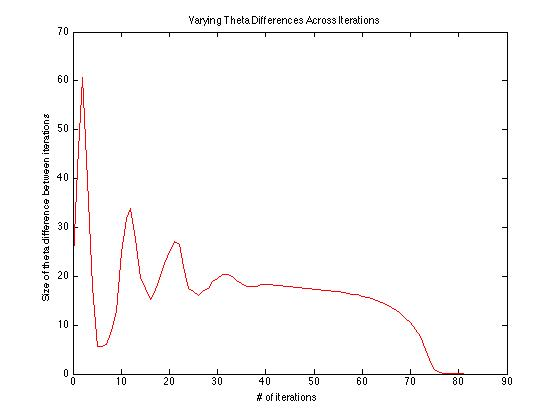
\includegraphics[scale=0.4]{theta_diff.jpg}
\end{figure}

It should be noted that if a smaller $\eta$ was chosen the plots 7-9 would have less oscillation within them.
It is also true that we could possible find a ``better'' solution if we allowed for smaller $\epsilon$, but it would take longer to converge.
A trade-off between speed and finding the best possible solution does exist with gradient descent.

\section{Problem 4}


\end{document}